
Having reviewed the fundamental concepts and the construction of DFAs across different rungs of the Jacob's ladder, in this section, we shall briefly review some of the key concepts that are related to both the numerical implementations and practical applications of DFT calculations.

\paragraph{\textbf{Self-consistent field (SCF)}} From \cref{eq:DFT_min_rho} and \cref{eq:KS_eqn}, it can be seen that, the solution of the Kohn-Sham equation provides us with the ground state single electron density $\rho(\bm{r})$ for a system with a fixed nuclei position. However, the construction of the Kohn-Sham energy functional itself requires the knowledge of $\rho(\bm{r})$, which is not known \emph{apriori}. This is seemingly like a `\emph{chicken-and-egg}' problem, Mathematically, such a problem can be tackled by computing the SCF in DFT, which is typically formulated by rewriting the Kohn-Sham energy in \cref{eq:KS_eqn} as its corresponding Kohn-Sham potential $V_{\scriptsize{\mbox{KS}}}(\bm{r})=[\delta E_{\scriptsize{\mbox{KS}}}(\bm{r})/\delta \rho]\vert_{\rho(\bm{r})}$. 

Practically, as shown in \cref{fig:KS-SCF}(left), the SCF starts with a initial guessed electron density $\rho_{0}(\bm{r})$ based on the crystal potential (here refer to a periodic calculation), that is determined by the positions of the nuclei. Then, the initial density $\rho_{0}$ can be used  as the input density $\rho^{\scriptsize{\mbox{in}}}$ to construct the effective Kohn-Sham potential $V_{\scriptsize{\mbox{KS}}}$ that can be plugged into the corresponding Kohn-Sham equation, solving which leads to an updated electron density $\rho^{\scriptsize{\mbox{out}}}$. By comparing the difference $\| \rho^{\scriptsize{\mbox{out}}}-\rho^{\scriptsize{\mbox{in}}}\|$, one can gauge if the input density correctly reflects the underlying crystal potential, and if the discrepancy between the two is large, then   $\rho^{\scriptsize{\mbox{out}}}$ will be refined (\emph{e.g.} with quasi-Newton method) and plugged back into the Kohn-Sham equation as the new $\rho^{\scriptsize{\mbox{in}}}$ to solve for a new $\rho^{\scriptsize{\mbox{out}}}$. This procedure will be carried out iteratively until $\| \rho^{\scriptsize{\mbox{out}}}-\rho^{\scriptsize{\mbox{in}}}\|$ is lower than a pre-defined convergence criteria. \cref{fig:KS-SCF}(right)\cite{woods2019computing} provides a schematic illustration on how the electron density evolves in an SCF procedure to reflect the underlying electrostatic potential. 
 
\begin{figure}[t] 
    \centering
    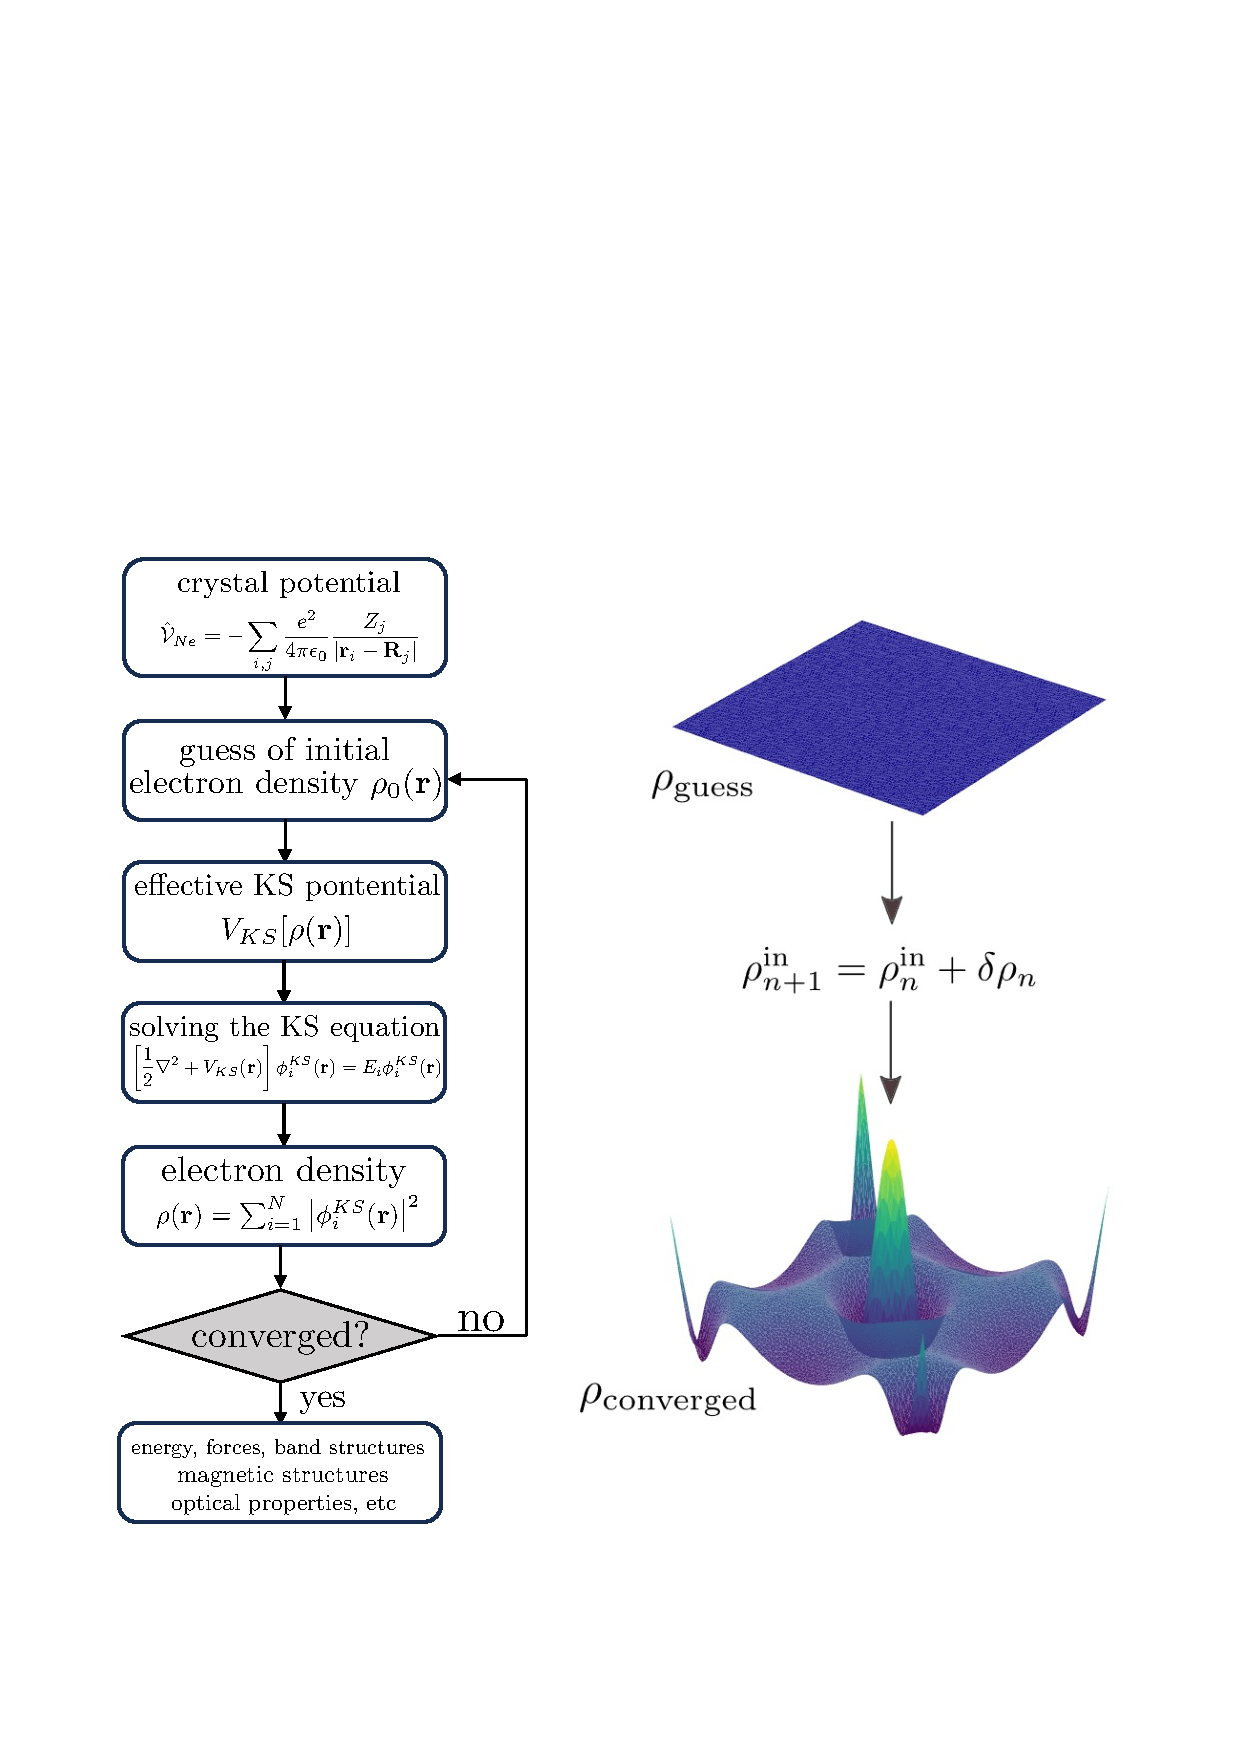
\includegraphics[width=0.6\textwidth]{KS-SCF.pdf}
    \caption{(left) Schematic flowchart for the self-consistent field procedure for solving the Kohn-Sham equation. (right) An iterative algorithm generates a series of perturbations to the density $\delta \rho_n$ in order to converge the initial guess density (top) to the fixed-point density $\rho_{*}$ (bottom). Example shown for an FCC four atom aluminium unit cell. [\citet{woods2019computing}]}
    \label{fig:KS-SCF}
\end{figure}

Because the SCF equation is solved iteratively to reach self-consistency, there are considerations that need to be accounted for, with corresponding approaches and methodologies being developed to address these issues to accelerate the convergence of electronic SCF in practical DFT calculations, which we will outline a few of them that occur commonly in the literature, whereas for more comprehensive discussion on SCF, we refer the readers to the review by \citet{woods2019computing}.

Firstly, the SCF procedure is aiming at searching for a local optimum of $\rho(\bm{r})$ under a given crystal potential $\hat{\mathcal{V}}_{Ne}$, and as in any local optimisation problem, the choice of the initial guess $\rho_0(\bm{r})$ plays an important role in how fast the algorithm can find the optimum solution. This is a particularly serious issue in spin-polarised Kohn-Sham calculations in which the spin-up [$\rho^\uparrow (\bm{r})$] and spin-down [$\rho^\downarrow (\bm{r})$] electron densities must be treated independently to determine the net spin polarisation of the system as $\rho^{\mbox{\scriptsize{spin}}}(\bm{r})=\rho^\uparrow(\bm{r})-\rho^\downarrow(\bm{r})$, in which the corresponding charge density $\rho^{\mbox{\scriptsize{charge}}}(\bm{r})=\rho^\uparrow(\bm{r})+\rho^\downarrow(\bm{r})$. This doubles the dimensionality of the search space and leads to slower or even difficulties in converging the SCF, compared to a spin non-polarised calculation, in which one can apply the constraint such that $\rho^{\mbox{\scriptsize{charge}}}(\bm{r})=2\rho^\uparrow(\bm{r})$. Practically, the slow convergence in spin-polarised calculations are usually remedied with two approaches by either using a converged  $\rho^{\mbox{\scriptsize{charge}}}(\bm{r})$ from non-spin-polarised calculation as the input for the subsequent spin-polarised calculation, or, if a particular spin-state (\emph{e.g.} ferromagnetic or antiferromagnetic) is desired, then the corresponding spin density on individual atom can be specified and used to construct $\rho_0 (\bm{r})$.

Secondly, it was found in the SCF procedure, that directly using $\rho^{\scriptsize{\mbox{out}}}_n$ from the $n$-th iteration as the input $\rho^{\scriptsize{\mbox{in}}}_{n+1}$ for the $(n+1)$-th interaction often led to numerical instability thus slow SCF convergence. A practical solution to this problem is to adapt a \emph{density-mixing} scheme, in which $\rho^{\scriptsize{\mbox{in}}}_{n+1}$ is constructed by proportionally mixing $\rho^{\scriptsize{\mbox{out}}}_{n}$ with the residues $\delta\rho_n=\|\rho^{\scriptsize{\mbox{out}}}_{n}-\rho^{\scriptsize{\mbox{in}}}_{n}\|$ from previous $n$ iterations. A similar approach in modern deep learning can be seen in the architecture of the residual multilayer perceptron (MLP) to accelerate model training.\cite{he2016deep} Some of the widely used density-mixing schemes in DFT include: (1) The Pulay scheme,\cite{pulay1980convergence} or otherwise known as Direct Inversion of the Iterative Subspace (DIIS), in which one seeks an ansatz $\rho_{n+1}^{\scriptsize{\mbox{in}}}=\sum_{i=n-m+1}^{n}c_i \rho^{\scriptsize{\mbox{out}}}_i$ as the linear combination of the output density $\rho^{\scriptsize{\mbox{out}}}_i$ from previous $m$ $(m<n)$ SCF interactions, with the coefficient $c_i$ being determined from minimising the weighted residue of $\|\sum_{i=n-m+1}^{n}c_i \delta\rho_i\|^2$. (2) The Broyden scheme,\cite{johnson1988modified,broyden1965class} further generalise the Pulay scheme. Generally, in a gradient-based optimisation, the function can be updated by using the relationship $\rho_{n+1}=\rho_{n}-\bm{J}_n^{-1}\delta \rho_n$ with $\bm{J}_n^{-1}$  being the inverse Jacobian matrix. However, direct calculation and inversion of the Jacobian matrix at each iteration is costly, and instead, according to \citet{broyden1965class}, one could initiate $\bm{J}_{0}^{-1}$ with a simple diagonal matrix and iteratively update it along with $\rho$ in the SCF procedure. Note that these mixing procedures are proposed as the general accelerating schemes for local optimisation problems, and are similarly applied to other problems in atomistic materials modelling, such as geometry optimisations.

Finally, the electron density is constructed from the Kohn-Sham orbitals as 
\begin{equation}
    \label{eq:electron_density_KS_orbital}
\rho(\bm{r})=\sum_{i=1}^{N}c_i|\phi^{\mbox{\scriptsize{KS}}}_i(\bm{r})|,
\end{equation}
in which $c_i=2$ and 0 for occupied and unoccupied non-spin-polarised orbitals at 0 K, respectively. Whilst this is physically correct, the discontinuity in the orbital occupations $c_i$ can lead to numerical instability in the SCF calculation. One solution to overcome this problem is to allow fractional occupancies by exciting electrons from the occupied to the unoccupied orbitals whilst satisfying the constraints of the exclusion principle, \emph{i.e.} $c_{i}\in [0,2]$, whilst $\sum_{i=1}^{N} c_i=N_e$, the total number of electrons in the system. For solid-state calculations, in particular, this may be achieved with Fermi smearing by introducing an electronic temperature $T_i$ such that $c_i=1/[\exp (\epsilon_i-\mu)/T+1]$ according to the Fermi-Dirac statistics, where $\mu$ is the Fermi energy.

\paragraph{\textbf{Basis functions}} One question that has not been addressed in the SCF procedure is how one should construct the Kohn-Sham orbitals $\{\varphi^{\mbox{\scriptsize{KS}}}_i(\bm{r})\}$ that leads to the electron density [\cref{eq:electron_density_KS_orbital}], which also determines how the electron density is algorithmically optimised to the one corresponding to the Kohn-Sham ground state. 

We answer this question by first looking at the case of molecular systems in the field of quantum chemistry, whereby the finite spatial extent of a molecule renders the corresponding SCF calculations to be performed with orbitals represented in real space, which is conceptually easy to understand. For this case, to be in line with the molecular orbital theory in physical chemistry that takes the molecular orbitals as the \emph{linear combination of atomic orbitals} (LCAO), we construct the Kohn-Sham orbital using \emph{atom-centred basis functions} $\{\varphi_{\mu}(\bm{r})\}$ such that 
\begin{equation}
\label{eq:molecular_basis_func_expansion}
\phi_i(\bm{r})=\sum_{\mu}c_{i\mu}\varphi_{\mu}(\bm{r}).
\end{equation}
Under such a construction, the SCF is essentially a procedure that iteratively adjusts the expansion coefficients $\{c_i,c_{i\mu}\}$ to reach the optimum $\rho(\bm{r})$ for a given molecule. A trivial choice for $\{\phi_{\mu}(\bm{r})$ is to follow the solution of hydrogen atom from the Schr\"{o}dinger equations by using a functional form of 
\begin{equation}
\varphi_{\mu}^{\mbox{{\scriptsize{Slater}}}}(r)\sim r^n e^{-\zeta r},
\end{equation}
which leads to the design of the Slater basis functions\cite{slater1930atomic} that gives the correct cusp and exponential decay behaviour with respect to $r$ as derived from fundamental quantum mechanics. However, the Slater basis functions are rarely used in modern quantum chemistry practices because the computation of the overlap integral [such as \cref{eq:exchange_HF_DFT}
 for the exact exchange] is difficult thus not numerically efficient. 

To overcome this problem, \citet{boys1950electronic} introduces the Gaussian basis set:
\begin{equation}
\varphi_{\mu}^{\mbox{{\scriptsize{Gaussian}}}}(r)\sim r^n e^{-\zeta r^2},
\end{equation}
which is now the standard choice in molecular calculations, for which the molecular integrals between two atomic orbitals can be analytically calculated. This significantly enhances the computational efficiency, however, the Gaussian basis function do not have the correct cusp and long-ranged decay behaviours as in the Slater's basis function. Solving this problem gave rise to the famous Pople basis functions\cite{hehre1969self}, in which a contraction scheme was devised to optimise a combination of the Gaussian functions to achieve a good approximation on the shape of a particular Slater orbital, while the numerical efficacy of the Gaussian basis functions could be retained, achieving the desirable outcomes from both the Slater and Gaussian basis functions. 

Theoretically, one can anticipate from  \cref{eq:molecular_basis_func_expansion} that the most accurate system energy can be acquired if the expansion is complete $\mu\to\infty$, which leads to the so-called complete basis set limit. However, this can never be achieved practically whereby the basis function must be truncated up to a certain order $\mu_{\max}$. In quantum chemical calculations on the non-covalent interaction energy between two fragments $\mathcal{A}$ and $\mathcal{B}$, this gives rise to the basis set superposition error (BSSE)\cite{boys1970calculation} in the computed interaction energy. Computing the interaction energy is usually achieve by computing the total energies for the isolated systems $\mathcal{A}$ and $\mathcal{B}$, as well as the interacting system $\mathcal{AB}$ first in the basis functions of $a\in\mathcal{A}$, $b\in\mathcal{B}$ and $a\cup b$ for $\mathcal{AB}$, respectively. From here we have [\emph{c.f.} \cref{eq:formation_energy}]:
\begin{equation}
    \Delta E(\mathcal{AB})=E^{a\cup b}(\mathcal{AB})-\left(E^{a}(\mathcal{A})+E^{b}(\mathcal{B}) \right).
\end{equation}
However, it can be seen from this expression that, when computing $E^{a\cup b}(\mathcal{AB})$, the computed energy of fragment $\mathcal{A}$ ($\mathcal{B}$) will be `contaminated' by the basis functions $b$ ($a$) from its interacting counterpart, since the size of the basis functions $a\cup b$ is larger than both $a$ and $b$, which is not the case when computing the terms $E^{a}(\mathcal{A})$ or $E^{b}(\mathcal{B})$. This generally results in the overbinding of the non-covalent complexes, and can be corrected by applying the counterpoise correction scheme.


\begin{wrapfigure}[30]{r}{0.35\textwidth}
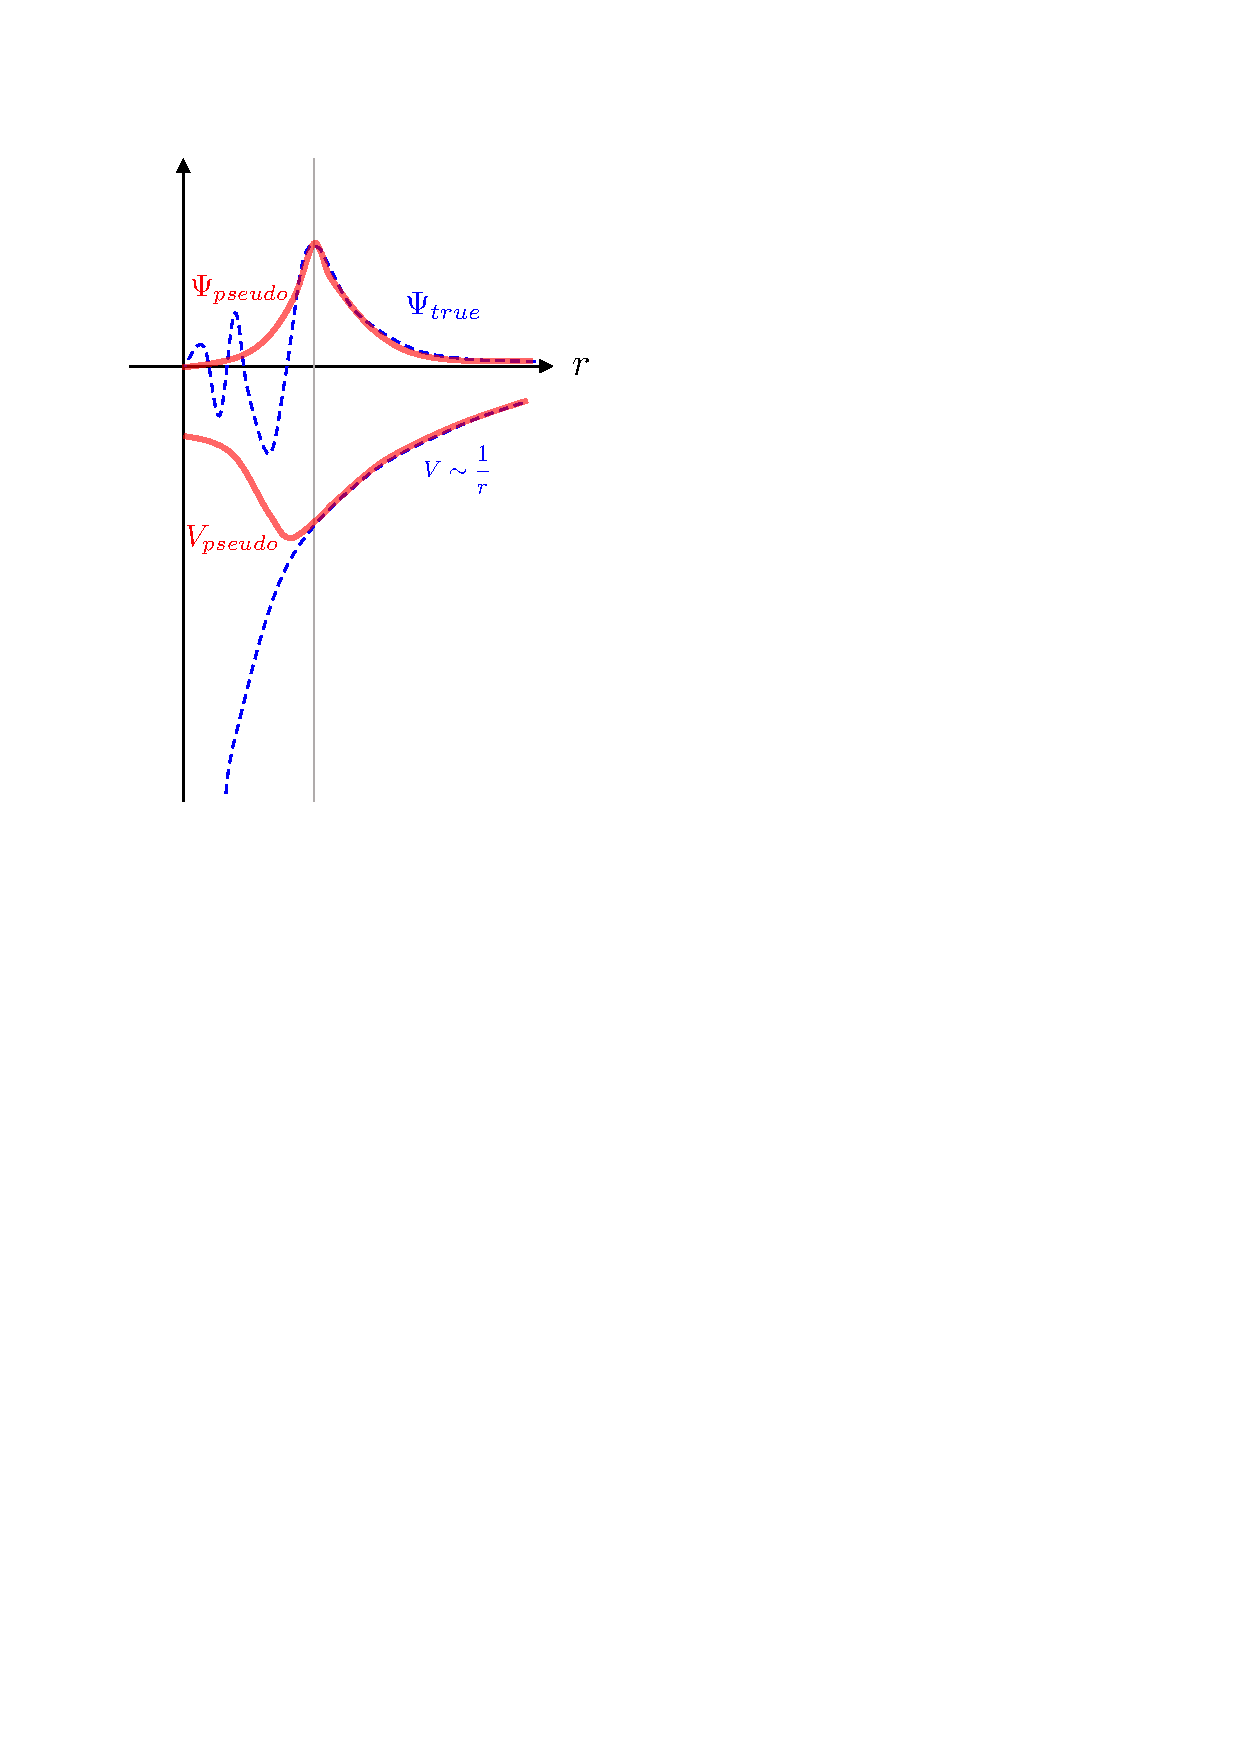
\includegraphics[width=0.35\textwidth]{pseudopotential.pdf}
\caption{Illustration of the construction of pseudopotential (red), which replaces the diverging Coulomb potential (blue) below the cut-off radius (grey solid line) with one  has finite value when $r\to 0$. This results in a pseudowavefunction that is more smooth and less oscillatory within the core region of an atom.}
   \label{fig:pseudopotential}
\end{wrapfigure}


For solid state calculations, on the other hand, one typically applies the planewave basis function in respect of the periodic boundary conditions. Based on the Bloch theory,  a suitable form of the planewave basis function can be written as 
\begin{equation}
    \label{eq:bloch_wave}
    \Psi_{n,\bm{k}}(\bm{r})=e^{i\bm{k}\cdot\bm{r}} u_{n,\bm{k}}(\bm{r})=\sum_{\bm{G}}c_{n,\bm{k}}(\bm{G}) e^{i(\bm{k+G})\cdot\bm{r}},
\end{equation}
in which $u_{n,\bm{k}}(\bm{r})$ is the wavefunction that reflects the local crystal potential and $\bm{G}$ is the reciprocal lattice vector. Similar to the situation in molecular calculations where the accuracy increases with the increasing sizes of basis set, in periodic calculations, the number of reciprocal lattice points included in $\{\bm{G}\}$ will dictate the accuracy of the simulation, which can be selected based on the cutoff of the electronic kinetic energy as $\frac{\hbar^2}{2m}|\bm{k}+\bm{G}|^2\leq E_{\mbox{\scriptsize{cutoff}}}^{\mbox{\scriptsize{kin}}}$. Unlike localised basis functions, because the planewave basis functions is fully delocalised in space, and the kinetic energy cutoff is also independent from the atomic positions, it does not suffer from BSSE for noncovalently bound systems, such as molecular crystals.


%\begin{figure}[tbh]   
%    \centering
%    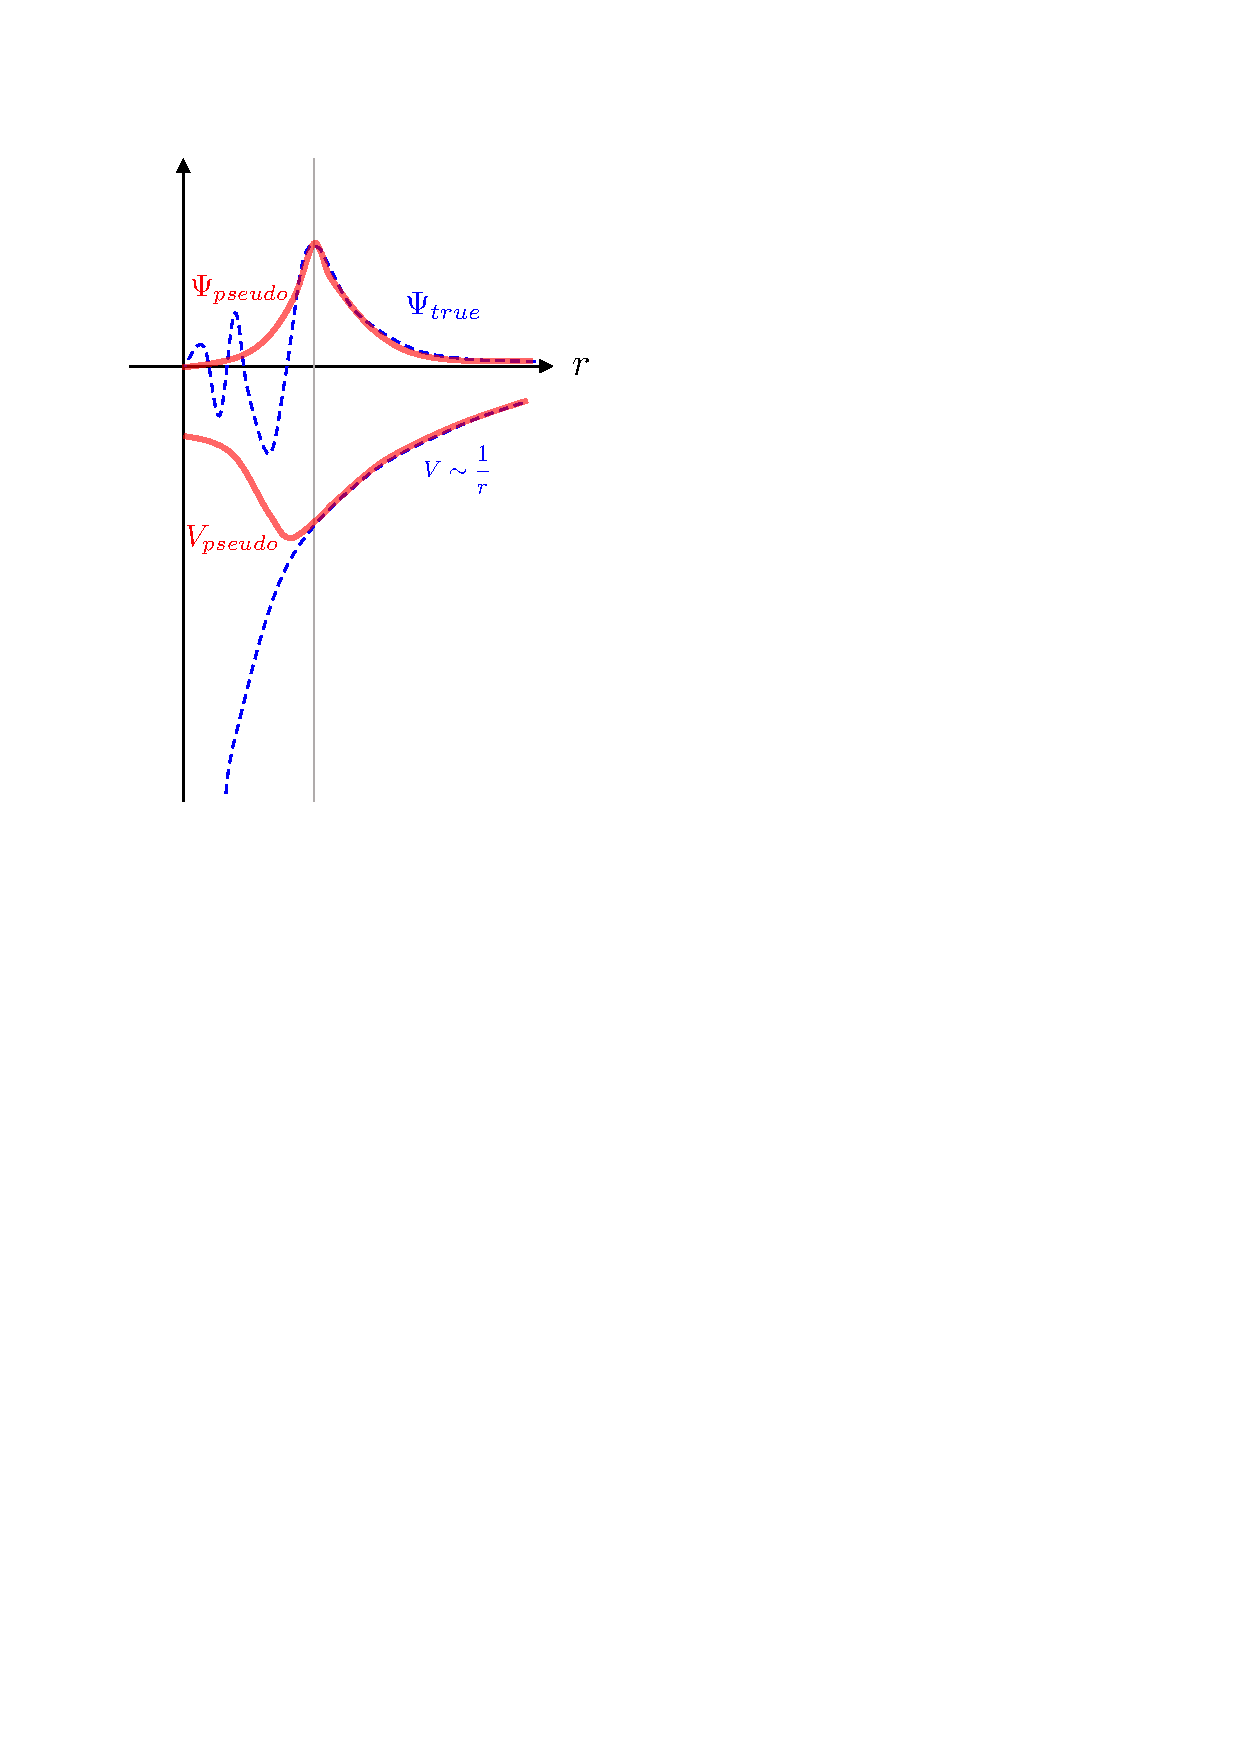
\includegraphics[width=0.4\textwidth]{pseudopotential.pdf}
 %   \caption{Illustration of the construction of pseudopotential (red), which replaces the diverging Coulomb potential (blue) below the cut-off radius (grey solid line) with one  has finite value when $r\to 0$. This results in a pseudowavefunction that is more smooth and less oscillatory within the core region of an atom.}
 %   \label{fig:pseudopotential}
%\end{figure}

Nevertheless, direct application of \cref{eq:bloch_wave} in implementing periodic DFT is not numerically efficient. This is because, close to the nuclei, the core electronic wavefunction typically exhibits wild oscillations, which require superpositioning many planewaves to correctly model this behaviour because a large $\bm{G}$ is needed to model core electrons with high $E^{\scriptsize{\mbox{kin}}}$.  This is not a problem when using the localised basis functions, in which both the core and valence electrons can be modelled with basis functions of the same form. In order to balance both the accuracy of all-electron calculations and the efficacy of planewave basis functions for periodic systems, the projector augmented wave (PAW)\cite{blochl1994projector} was proposed and has been a successful scheme that is adopted, for example, in the widely used planewave DFT code VASP (Vienna \emph{ab initio} Simulation Package).\cite{kresse1996efficient} In its essence, the PAW is constructed as follows
\begin{equation}
    \label{eq:PAW}
    \left|\Psi\right\rangle=\left(|\bar{\Psi}\rangle - \sum_i |\tilde{\phi}_i\rangle \langle\tilde{p}_i|\bar{\Psi}\rangle\right) + \sum_i |\phi_i\rangle \langle\tilde{p}_i|\bar{\Psi}\rangle,
\end{equation}
in which $|\bar{\Psi}\rangle$ represents the pseudo wavefunction that is expanded in the planewave basis, $|\phi_i\rangle$ and $|\tilde{\phi}\rangle$ are the pseudo wavefunction for valence and core electrons in a localised basis, respectively. Finally $\langle\tilde{p}_i|$ is a projector function. With this, the bracketed term in \cref{eq:PAW} removes the part in the planewave that is suppose to model the core electronic behaviour, that is subsequently replaced by [remaining term in \cref{eq:PAW}]  an oscillating core-like wavefunction that is projected onto the planewave basis.



\paragraph{\textbf{Pseudopotentials}}  To further overcome the problem of having to use a large number of $\bm{G}$ vectors in the reciprocal space for expanding the core electron wavefunctions with the planewave basis functions, we utilise the fact that, in comparison with the spatially delocalised valence electrons, the core electrons play a minimal role in determining the chemical bondings and electronic properties of materials. This means that in practical DFT calculations, one only needs to model the behaviours of core electrons approximately. This leads to the concept and developments of pseudopotentials that are often applied in conjunctions with the planewave basis functions in DFT calculations for periodic solids.



\cref{fig:pseudopotential} provides an illustration on the core idea behind the atomic pseudopotential $V_{\mathrm{pseudo}}(\bm{r})$, which is a smoothly varying potential, such that below the core/valence cut-off distance $r_c$, $V_{\mathrm{pseudo}}(\bm{r})$ varies slowly to a finite value as $\|r\|\to0$, instead of diverging to $-\infty$ as for the case of a true Coulomb electrostatic potential generated from the positively charged nuclei. On the other hand, when $\bm{r}>\bm{r}_c$, $V_{\mathrm{pseudo}}(\bm{r})$ resembles the original form of the Coulomb potential for a particular atom. Consequently, the pseudowavefunction $\Psi_{\mathrm{pseudo}}(\bm{r})$ that is solved from the Schr\"{o}dinger equation with $V_{\mathrm{pseudo}}(\bm{r})$ should become a slowly varying one when $\bm{r}<\bm{r}_c$, while resembling the correct tailing wavefunction in the valence region, as if the original Coulomb potential was used.  Here, we will briefly review the two major categories of the constructions for the pseudopotentials that are widely used in the community.

The \emph{norm-conserving pseudopotentials}\cite{hamann1979norm,vanderbilt1985optimally,hamann2013optimized} are constructed by directly applying the concept discussed above through imposing the constraint such that the norm of the pseudowavefunction $\Psi_{\mathrm{pseudo}}(\bm{r})$ within the cut-off distance should equal to that of an all-electron wavefunction $\phi_{\mathrm{all-electron}}(\bm{r})$,  \emph{i.e.}
\begin{equation}\label{eq:norm_conserve_constraint}
    \int_0^{\bm{r}_c}\left\|\Psi_{\mathrm{pseudo}}(\bm{r})\right\|^2 \mbox{d}\bm{r} = \int_0^{\bm{r}_c}\left\|\phi_{\mathrm{all-electron}}(\bm{r})\right\|^2 \mbox{d}\bm{r}.
\end{equation}
Additionally, $\Psi_{\mathrm{pseudo}}(\bm{r})$ needs to be a continuous and differentiable function at $\bm{r}_c$. Typically the all electron wavefunction for each orbital (based on the quantum number $\ell$) is first solved for a given atom with, for example, localised basis function, which allows one to fit a corresponding $\Psi_{\mathrm{pseudo}}^{\ell}(\bm{r})$ under the norm-conservation constraint. To obtain the final pseudopotential, we note that $\Psi_{\mathrm{pseudo}}^{\ell}(\bm{r})$ should satisfy the following Schr\"{o}dinger equation:
\begin{equation*}
    \left[-\frac{1}{2}\nabla^2_{\bm{r}} +\frac{\ell(\ell+1)}{2r^2}+V_{\mathrm{pseudo}}^\ell(\bm{r})\right]\Psi^{\ell}(\bm{r})=\varepsilon_\ell  \Psi^{\ell}(\bm{r}).
\end{equation*}
By harnessing the linearity of the Schr\"{o}dinger equation, we can compute the corresponding pseudopotential from $\Psi^{\ell}(r)$ and $\varepsilon_\ell$ directly as:
\begin{equation*}
    \label{eq:norm_conserved_PP}
    V_{pseudo}^\ell (\bm{r}) = \varepsilon_\ell+\frac{1}{2\Psi^\ell (\bm{r})}\nabla^2_{\bm{r}} \Psi^{\ell}(\bm{r})-\frac{\ell(\ell+1)}{2r^2}.
\end{equation*}
While this is conceptually simple, the pseudowavefunction $\Psi_{\mathrm{pseudo}}(\bm{r})$ that is produced under the norm-conserving constraint can still retain significant oscillatory behaviours, such that the problem of large $\bm{G}$ vector needed in constructing the  planewave basis function cannot be fully circumvented, particularly for transition metals with very localised valence states.

The \emph{ultrasoft pseudopotentials}\cite{laasonen1991implementation,kresse1999ultrasoft} were introduced to further overcome the problem in the norm-conserving pseudopotentials by lowering the energy cutoff to enhance the computational efficiencies. It achieves this by  relaxing the norm-conserving condition [\cref{eq:norm_conserve_constraint}] to achieve a smoother $\Psi_{\mathrm{pseudo}}(\bm{r})$ through allowing less charge density to be retained within the core region whilst preserving the total electron density of a given atom, which means now the constraint [\cref{eq:norm_conserve_constraint}] should be rewritten as:
\begin{equation}
    \label{eq:ultrasoft_PP_charge_constraint}
    \Delta \rho=\int_0^\infty \left(\Psi^* (\bm{r})\Psi(\bm{r})-\phi^*(\bm{r})\phi(\bm{r})\right)\mbox{d}\bm{r}\to 0.
\end{equation}
Because the pseudowavefunction $\Psi_{\mathrm{pseudo}}(\bm{r})$ is very smooth, it generally cannot preserve the total charge of an atom. The solution proposed for this problem is to reconstruct the total charge density by rewritting the total atomic charge density as:
\begin{equation*}
    \rho(\bm{r})=\sum_{i}f_i \|\phi_i (\bm{r})\|^2+\rho^{\mbox{\scriptsize{aug}}}(\bm{r}),
\end{equation*}
in which $f_i$ is the atomic orbital occupation number. The augmented electron density $\rho^{\mbox{\scriptsize{aug}}}(\bm{r})=\sum_{ij}q_{ij}Q_{ij}(\bm{r})$ effectively projects the differences in the total charge densities calculated from localised and planewave basis functions, \emph{i.e.} $Q_{ij}(\bm{r})=\phi_{i}^{*}(\bm{r})\phi_{j}(\bm{r})-\Psi_{i}^{*}(\bm{r})\Psi_{j}(\bm{r})$, onto the localised basis function with $q_{ij}=\sum_n f_n \langle \phi_n|\beta_i\rangle\langle\beta_j |\phi_n\rangle$, with $|\beta_i\rangle$ being a projector operator that depends on $\phi_i$. Essentially $\rho^{\mbox{\scriptsize{aug}}}(\bm{r})$ measures how much charge density is missing when a particular atomic orbital is relaxed from $\phi$ to its corresponding $\Psi$. Unlike the norm-conserving pseudopotentials, the formulation for the ultrasoft pseudopotential does not give a potential directly, but rather the ingredients to reconstruct the Kohn-Sham equations to solve for the corresponding Kohn-Sham orbitals:
\begin{equation*}
    %\label{eq:ultrasoft_PP_KS_eqn}
    \left[-\frac{1}{2}\nabla^2+\hat{V}_{local}+\hat{V}_{NL}\right]\psi_n^{\mbox{\scriptsize{KS}}}=\varepsilon_n  \hat{S} \psi_n^{\mbox{\scriptsize{KS}}}.
\end{equation*}
Here, the local potential $\hat{V}_{local}$ contains the Hartree, exchange-correlation and ionic contributions that can be obtained from $\rho(\bm{r})$ by solving the Poisson equation. The non-local potential is given by the projector $\hat{V}_{NL}=\sum_{ij}D_{ij}|\beta_i\rangle\langle\beta_j|$, in which $D_{ij}$ is the non-local potential coefficient obtained by matching the eigenvalues of the pseudo atomic wavefunction to its true wavefunction. Finally, $\hat{S}=1+\sum_{ij}q_{ij}|\beta_i\rangle\langle\beta_j|$ is the orbital overlap operator. 

The development and wide adaption of pseudopotentials have undoubtedly become an inseparable factor for the success of DFT in material chemistry and physics. However, as in any approximations proposed to simplify the practical implementation of the theory, it also comes with its own limitations. Firstly,  by approximating the core electrons in pseudopotentials prevents accurate modelling of physical effects in which core electrons can also play a critical role, such as spin-orbit coupling,\cite{dolg2012relativistic} high-pressure physics,\cite{oganov2003all} and core-level spectroscopies. Secondly, because the targets for fitting the pseudopotentials are the  orbitals of individual isolated atoms, it cannot reflects the change in the atomic potential due to the neighbouring bonding environments, which could reduce their transferabilities. Thirdly, as one can see in the formulation of the ultrasoft pseudopotential, its practical implementation is directly tightened up with the corresponding implementation of the Kohn-Sham equation, which can further limit its  transferability across different DFT codes.   
 